% Options for packages loaded elsewhere
% Options for packages loaded elsewhere
\PassOptionsToPackage{unicode}{hyperref}
\PassOptionsToPackage{hyphens}{url}
\PassOptionsToPackage{dvipsnames,svgnames,x11names}{xcolor}
%
\documentclass[
  letterpaper,
  12pt,
  twoside]{reedthesis}
\usepackage{xcolor}
\usepackage{amsmath,amssymb}
\setcounter{secnumdepth}{5}
\usepackage{iftex}
\ifPDFTeX
  \usepackage[T1]{fontenc}
  \usepackage[utf8]{inputenc}
  \usepackage{textcomp} % provide euro and other symbols
\else % if luatex or xetex
  \usepackage{unicode-math} % this also loads fontspec
  \defaultfontfeatures{Scale=MatchLowercase}
  \defaultfontfeatures[\rmfamily]{Ligatures=TeX,Scale=1}
\fi
\usepackage{lmodern}
\ifPDFTeX\else
  % xetex/luatex font selection
\fi
% Use upquote if available, for straight quotes in verbatim environments
\IfFileExists{upquote.sty}{\usepackage{upquote}}{}
\IfFileExists{microtype.sty}{% use microtype if available
  \usepackage[]{microtype}
  \UseMicrotypeSet[protrusion]{basicmath} % disable protrusion for tt fonts
}{}
\makeatletter
\@ifundefined{KOMAClassName}{% if non-KOMA class
  \IfFileExists{parskip.sty}{%
    \usepackage{parskip}
  }{% else
    \setlength{\parindent}{0pt}
    \setlength{\parskip}{6pt plus 2pt minus 1pt}}
}{% if KOMA class
  \KOMAoptions{parskip=half}}
\makeatother
% Make \paragraph and \subparagraph free-standing
\makeatletter
\ifx\paragraph\undefined\else
  \let\oldparagraph\paragraph
  \renewcommand{\paragraph}{
    \@ifstar
      \xxxParagraphStar
      \xxxParagraphNoStar
  }
  \newcommand{\xxxParagraphStar}[1]{\oldparagraph*{#1}\mbox{}}
  \newcommand{\xxxParagraphNoStar}[1]{\oldparagraph{#1}\mbox{}}
\fi
\ifx\subparagraph\undefined\else
  \let\oldsubparagraph\subparagraph
  \renewcommand{\subparagraph}{
    \@ifstar
      \xxxSubParagraphStar
      \xxxSubParagraphNoStar
  }
  \newcommand{\xxxSubParagraphStar}[1]{\oldsubparagraph*{#1}\mbox{}}
  \newcommand{\xxxSubParagraphNoStar}[1]{\oldsubparagraph{#1}\mbox{}}
\fi
\makeatother

\usepackage{color}
\usepackage{fancyvrb}
\newcommand{\VerbBar}{|}
\newcommand{\VERB}{\Verb[commandchars=\\\{\}]}
\DefineVerbatimEnvironment{Highlighting}{Verbatim}{commandchars=\\\{\}}
% Add ',fontsize=\small' for more characters per line
\usepackage{framed}
\definecolor{shadecolor}{RGB}{241,243,245}
\newenvironment{Shaded}{\begin{snugshade}}{\end{snugshade}}
\newcommand{\AlertTok}[1]{\textcolor[rgb]{0.68,0.00,0.00}{#1}}
\newcommand{\AnnotationTok}[1]{\textcolor[rgb]{0.37,0.37,0.37}{#1}}
\newcommand{\AttributeTok}[1]{\textcolor[rgb]{0.40,0.45,0.13}{#1}}
\newcommand{\BaseNTok}[1]{\textcolor[rgb]{0.68,0.00,0.00}{#1}}
\newcommand{\BuiltInTok}[1]{\textcolor[rgb]{0.00,0.23,0.31}{#1}}
\newcommand{\CharTok}[1]{\textcolor[rgb]{0.13,0.47,0.30}{#1}}
\newcommand{\CommentTok}[1]{\textcolor[rgb]{0.37,0.37,0.37}{#1}}
\newcommand{\CommentVarTok}[1]{\textcolor[rgb]{0.37,0.37,0.37}{\textit{#1}}}
\newcommand{\ConstantTok}[1]{\textcolor[rgb]{0.56,0.35,0.01}{#1}}
\newcommand{\ControlFlowTok}[1]{\textcolor[rgb]{0.00,0.23,0.31}{\textbf{#1}}}
\newcommand{\DataTypeTok}[1]{\textcolor[rgb]{0.68,0.00,0.00}{#1}}
\newcommand{\DecValTok}[1]{\textcolor[rgb]{0.68,0.00,0.00}{#1}}
\newcommand{\DocumentationTok}[1]{\textcolor[rgb]{0.37,0.37,0.37}{\textit{#1}}}
\newcommand{\ErrorTok}[1]{\textcolor[rgb]{0.68,0.00,0.00}{#1}}
\newcommand{\ExtensionTok}[1]{\textcolor[rgb]{0.00,0.23,0.31}{#1}}
\newcommand{\FloatTok}[1]{\textcolor[rgb]{0.68,0.00,0.00}{#1}}
\newcommand{\FunctionTok}[1]{\textcolor[rgb]{0.28,0.35,0.67}{#1}}
\newcommand{\ImportTok}[1]{\textcolor[rgb]{0.00,0.46,0.62}{#1}}
\newcommand{\InformationTok}[1]{\textcolor[rgb]{0.37,0.37,0.37}{#1}}
\newcommand{\KeywordTok}[1]{\textcolor[rgb]{0.00,0.23,0.31}{\textbf{#1}}}
\newcommand{\NormalTok}[1]{\textcolor[rgb]{0.00,0.23,0.31}{#1}}
\newcommand{\OperatorTok}[1]{\textcolor[rgb]{0.37,0.37,0.37}{#1}}
\newcommand{\OtherTok}[1]{\textcolor[rgb]{0.00,0.23,0.31}{#1}}
\newcommand{\PreprocessorTok}[1]{\textcolor[rgb]{0.68,0.00,0.00}{#1}}
\newcommand{\RegionMarkerTok}[1]{\textcolor[rgb]{0.00,0.23,0.31}{#1}}
\newcommand{\SpecialCharTok}[1]{\textcolor[rgb]{0.37,0.37,0.37}{#1}}
\newcommand{\SpecialStringTok}[1]{\textcolor[rgb]{0.13,0.47,0.30}{#1}}
\newcommand{\StringTok}[1]{\textcolor[rgb]{0.13,0.47,0.30}{#1}}
\newcommand{\VariableTok}[1]{\textcolor[rgb]{0.07,0.07,0.07}{#1}}
\newcommand{\VerbatimStringTok}[1]{\textcolor[rgb]{0.13,0.47,0.30}{#1}}
\newcommand{\WarningTok}[1]{\textcolor[rgb]{0.37,0.37,0.37}{\textit{#1}}}

\usepackage{longtable,booktabs,array}
\usepackage{calc} % for calculating minipage widths
% Correct order of tables after \paragraph or \subparagraph
\usepackage{etoolbox}
\makeatletter
\patchcmd\longtable{\par}{\if@noskipsec\mbox{}\fi\par}{}{}
\makeatother
% Allow footnotes in longtable head/foot
\IfFileExists{footnotehyper.sty}{\usepackage{footnotehyper}}{\usepackage{footnote}}
\makesavenoteenv{longtable}
\usepackage{graphicx}
\makeatletter
\newsavebox\pandoc@box
\newcommand*\pandocbounded[1]{% scales image to fit in text height/width
  \sbox\pandoc@box{#1}%
  \Gscale@div\@tempa{\textheight}{\dimexpr\ht\pandoc@box+\dp\pandoc@box\relax}%
  \Gscale@div\@tempb{\linewidth}{\wd\pandoc@box}%
  \ifdim\@tempb\p@<\@tempa\p@\let\@tempa\@tempb\fi% select the smaller of both
  \ifdim\@tempa\p@<\p@\scalebox{\@tempa}{\usebox\pandoc@box}%
  \else\usebox{\pandoc@box}%
  \fi%
}
% Set default figure placement to htbp
\def\fps@figure{htbp}
\makeatother


% definitions for citeproc citations
\NewDocumentCommand\citeproctext{}{}
\NewDocumentCommand\citeproc{mm}{%
  \begingroup\def\citeproctext{#2}\cite{#1}\endgroup}
\makeatletter
 % allow citations to break across lines
 \let\@cite@ofmt\@firstofone
 % avoid brackets around text for \cite:
 \def\@biblabel#1{}
 \def\@cite#1#2{{#1\if@tempswa , #2\fi}}
\makeatother
\newlength{\cslhangindent}
\setlength{\cslhangindent}{1.5em}
\newlength{\csllabelwidth}
\setlength{\csllabelwidth}{3em}
\newenvironment{CSLReferences}[2] % #1 hanging-indent, #2 entry-spacing
 {\begin{list}{}{%
  \setlength{\itemindent}{0pt}
  \setlength{\leftmargin}{0pt}
  \setlength{\parsep}{0pt}
  % turn on hanging indent if param 1 is 1
  \ifodd #1
   \setlength{\leftmargin}{\cslhangindent}
   \setlength{\itemindent}{-1\cslhangindent}
  \fi
  % set entry spacing
  \setlength{\itemsep}{#2\baselineskip}}}
 {\end{list}}
\usepackage{calc}
\newcommand{\CSLBlock}[1]{\hfill\break\parbox[t]{\linewidth}{\strut\ignorespaces#1\strut}}
\newcommand{\CSLLeftMargin}[1]{\parbox[t]{\csllabelwidth}{\strut#1\strut}}
\newcommand{\CSLRightInline}[1]{\parbox[t]{\linewidth - \csllabelwidth}{\strut#1\strut}}
\newcommand{\CSLIndent}[1]{\hspace{\cslhangindent}#1}



\setlength{\emergencystretch}{3em} % prevent overfull lines

\providecommand{\tightlist}{%
  \setlength{\itemsep}{0pt}\setlength{\parskip}{0pt}}



 


% Reed College Thesis Preamble for Quarto
% This supplements reedthesis.cls - only adds packages/features not in the class

% Additional packages (only those not loaded by Quarto or reedthesis.cls)
\usepackage{graphicx,latexsym}
\usepackage{amssymb,amsthm}
\usepackage{setspace}
\usepackage[hyphens]{url}
\usepackage{float}
% Use htbp (here, top, bottom, page) so LaTeX can choose the best placement.
% Avoid H (forced here) which causes large white gaps when a float doesn't fit.
\floatplacement{figure}{htbp}
\floatplacement{table}{htbp}
\usepackage{rotating}

% Caption formatting
\usepackage{caption}
\captionsetup{width=5in}

% Paragraph formatting to match Reed thesis style
\setlength{\parskip}{0pt}
\setlength{\parindent}{0.5in}

% Remove hyperlink colors to match traditional Reed thesis style (no colored links)
\AtBeginDocument{%
  \hypersetup{hidelinks}%
}

% Bibliography formatting - redefine CSLReferences for Reed thesis style
% Must redefine entirely because Quarto's definition sets itemsep inside the list
\renewenvironment{CSLReferences}[2]
 {\begin{list}{}{%
  \setlength{\itemindent}{0pt}%
  \setlength{\leftmargin}{0pt}%
  \setlength{\parsep}{0pt}%
  % turn on hanging indent if param 1 is 1
  \ifodd #1
   \setlength{\leftmargin}{\cslhangindent}%
   \setlength{\itemindent}{-1\cslhangindent}%
  \fi
  % Reed thesis style: add spacing between bibliography entries
  \setlength{\itemsep}{12pt plus 2pt minus 2pt}%
  }}
 {\end{list}}
\title{My Final College Paper}
\author{Your R. Name}
\date{May 2026}
\institution{Reed College}
\division{Mathematical and Natural Sciences}
\department{Mathematics}
\advisor{Advisor F. Name}
\degree{Bachelor of Arts}
\makeatletter
\@ifpackageloaded{bookmark}{}{\usepackage{bookmark}}
\makeatother
\makeatletter
\@ifpackageloaded{caption}{}{\usepackage{caption}}
\AtBeginDocument{%
\ifdefined\contentsname
  \renewcommand*\contentsname{Table of contents}
\else
  \newcommand\contentsname{Table of contents}
\fi
\ifdefined\listfigurename
  \renewcommand*\listfigurename{List of Figures}
\else
  \newcommand\listfigurename{List of Figures}
\fi
\ifdefined\listtablename
  \renewcommand*\listtablename{List of Tables}
\else
  \newcommand\listtablename{List of Tables}
\fi
\ifdefined\figurename
  \renewcommand*\figurename{Figure}
\else
  \newcommand\figurename{Figure}
\fi
\ifdefined\tablename
  \renewcommand*\tablename{Table}
\else
  \newcommand\tablename{Table}
\fi
}
\@ifpackageloaded{float}{}{\usepackage{float}}
\floatstyle{ruled}
\@ifundefined{c@chapter}{\newfloat{codelisting}{h}{lop}}{\newfloat{codelisting}{h}{lop}[chapter]}
\floatname{codelisting}{Listing}
\newcommand*\listoflistings{\listof{codelisting}{List of Listings}}
\makeatother
\makeatletter
\makeatother
\makeatletter
\@ifpackageloaded{caption}{}{\usepackage{caption}}
\@ifpackageloaded{subcaption}{}{\usepackage{subcaption}}
\makeatother
\usepackage{bookmark}
\IfFileExists{xurl.sty}{\usepackage{xurl}}{} % add URL line breaks if available
\urlstyle{same}
\hypersetup{
  pdftitle={My Final College Paper},
  pdfauthor={Your R. Name},
  colorlinks=true,
  linkcolor={blue},
  filecolor={Maroon},
  citecolor={Blue},
  urlcolor={Blue},
  pdfcreator={LaTeX via pandoc}}


\title{My Final College Paper}
\author{Your R. Name}
\date{May 2026}
\begin{document}
\maketitle

% Reed College Thesis - Before Body Content
% This is called after \begin{document}
% Note: \maketitle is called by Quarto's template, which will use reedthesis.cls
% to generate the proper title page and approval page with horizontal rules.

% Front matter with roman numerals and no page numbers shown
\frontmatter
\pagestyle{empty}

% Front matter content (acknowledgements, preface, TOC, LOT, LOF, abstract, dedication)
% is injected by the thesis-meta Lua filter based on YAML metadata


\begin{acknowledgements}
I want to thank a few people.
\end{acknowledgements}

\begin{preface}
This is an example of a thesis setup to use the Reed thesis document class (for LaTeX) and Quarto.
\end{preface}

\renewcommand{\contentsname}{Table of Contents}
\tableofcontents

\listoftables

\listoffigures

\begin{abstract}
This is your abstract text. You can write it here directly. It can span multiple paragraphs.
\end{abstract}

\begin{dedication}
You can have a dedication here if you wish.
\end{dedication}

\mainmatter
\pagestyle{fancyplain}

\bookmarksetup{startatroot}

\chapter*{Introduction}\label{introduction}
\addcontentsline{toc}{chapter}{Introduction}

\markboth{Introduction}{Introduction}

Welcome to the \emph{Quarto} thesis template. This template is based on
the Reed College LaTeX template, but provides a nicer interface for
those that have never used TeX or LaTeX before. Using \emph{Quarto} will
also allow you to easily keep track of your analyses in \textbf{R} or
\textbf{Python} code chunks, with the resulting plots and output
included as well. The hope is this \emph{Quarto} template gets you in
the habit of doing reproducible research, which benefits you long-term
as a researcher, but also will greatly help anyone that is trying to
reproduce or build onto your results down the road.

Hopefully, you won't have much of a learning period to go through and
you will reap the benefits of a nicely formatted thesis. The use of
LaTeX in combination with \emph{Markdown} is more consistent than the
output of a word processor, much less prone to corruption or crashing,
and the resulting file is smaller than a Word file. While you may have
never had problems using Word in the past, your thesis is likely going
to be about twice as large and complex as anything you've written
before, taxing Word's capabilities. After working with \emph{Quarto} for
a few weeks, we are confident this will be your reporting style of
choice going forward.

\textbf{Why use it?}

\emph{Quarto} creates a simple and straightforward way to interface with
the beauty of LaTeX. In addition to creating a user friendly interface
to LaTeX, \emph{Quarto} also allows you to read in your data, analyze
it, and visualize it using \textbf{R} or \textbf{Python}, and also to
provide the documentation and commentary on the results of your project.
Further, it allows for computed results to be passed inline to the
commentary of your results. You'll see more on this later.

\textbf{Who should use it?}

Anyone who needs to use data analysis, math, tables, a lot of figures,
complex cross-references, or who just cares about the final appearance
of their document should use \emph{Quarto}. Of particular use should be
anyone in the sciences, but the user-friendly nature of \emph{Markdown}
and its ability to keep track of and easily include figures,
automatically generate a table of contents, index, references, table of
figures, etc. should make it of great benefit to nearly anyone writing a
thesis project.

\textbf{For additional help with Quarto} Please visit
\href{https://quarto.org/docs/guide/}{the Quarto documentation}.

\bookmarksetup{startatroot}

\chapter{Quarto Basics}\label{rmd-basics}

Here is a brief introduction into using \emph{Quarto}. \emph{Markdown}
is a simple formatting syntax for authoring HTML, PDF, and MS Word
documents. \emph{Quarto} provides the flexibility of \emph{Markdown}
with the implementation of \textbf{R} (or Python) input and output. For
more details on using \emph{Quarto} see \url{https://quarto.org}.

Be careful with your spacing in \emph{Markdown} documents. While
whitespace largely is ignored, it does at times give \emph{Markdown}
signals as to how to proceed. As a habit, try to keep everything left
aligned whenever possible, especially as you type a new paragraph. In
other words, there is no need to indent basic text in the qmd document
(in fact, it might cause your text to do funny things if you do).

\section{Lists}\label{lists}

It's easy to create a list. It can be unordered like

\begin{itemize}
\tightlist
\item
  Item 1
\item
  Item 2
\end{itemize}

or it can be ordered like

\begin{enumerate}
\def\labelenumi{\arabic{enumi}.}
\tightlist
\item
  Item 1
\item
  Item 2
\end{enumerate}

Notice that I intentionally mislabeled Item 2 as number 4.
\emph{Markdown} automatically figures this out! You can put any numbers
in the list and it will create the list. Check it out below.

To create a sublist, just indent the values a bit (at least four spaces
or a tab). (Here's one case where indentation is key!)

\begin{enumerate}
\def\labelenumi{\arabic{enumi}.}
\tightlist
\item
  Item 1
\item
  Item 2
\item
  Item 3

  \begin{itemize}
  \tightlist
  \item
    Item 3a
  \item
    Item 3b
  \end{itemize}
\end{enumerate}

\section{Line breaks}\label{line-breaks}

Make sure to add white space between lines if you'd like to start a new
paragraph. Look at what happens below in the outputted document if you
don't:

Here is the first sentence. Here is another sentence. Here is the last
sentence to end the paragraph. This should be a new paragraph.

\emph{Now for the correct way:}

Here is the first sentence. Here is another sentence. Here is the last
sentence to end the paragraph.

This should be a new paragraph.

\section{R chunks}\label{r-chunks}

When you click the \textbf{Render} button (or run
\texttt{quarto\ render} from the terminal), a document will be generated
that includes both content as well as the output of any embedded
\textbf{R} code chunks within the document. You can embed an \textbf{R}
code chunk like this (\texttt{cars} is a built-in \textbf{R} dataset):

\begin{Shaded}
\begin{Highlighting}[]
\FunctionTok{summary}\NormalTok{(cars)}
\end{Highlighting}
\end{Shaded}

\begin{verbatim}
     speed           dist       
 Min.   : 4.0   Min.   :  2.00  
 1st Qu.:12.0   1st Qu.: 26.00  
 Median :15.0   Median : 36.00  
 Mean   :15.4   Mean   : 42.98  
 3rd Qu.:19.0   3rd Qu.: 56.00  
 Max.   :25.0   Max.   :120.00  
\end{verbatim}

\section{Inline code}\label{inline-code}

If you'd like to put the results of your analysis directly into your
discussion, add inline code like this:

\begin{quote}
The \texttt{cos} of \(2 \pi\) is 1.
\end{quote}

Another example would be the direct calculation of the standard
deviation:

\begin{quote}
The standard deviation of \texttt{speed} in \texttt{cars} is 5.2876444.
\end{quote}

One last neat feature is the use of the \texttt{ifelse} conditional
statement which can be used to output text depending on the result of an
\textbf{R} calculation:

\begin{quote}
The standard deviation is less than 6.
\end{quote}

Note the use of \texttt{\textgreater{}} here, which signifies a
quotation environment that will be indented.

As you see with \texttt{\$2\ \textbackslash{}pi\$} above, mathematics
can be added by surrounding the mathematical text with dollar signs.
More examples of this are in Mathematics and Science if you uncomment
the code in Math.

\section{Including plots}\label{including-plots}

You can also embed plots. For example, here is a way to use the base
\textbf{R} graphics package to produce a plot using the built-in
\texttt{pressure} dataset:

\pandocbounded{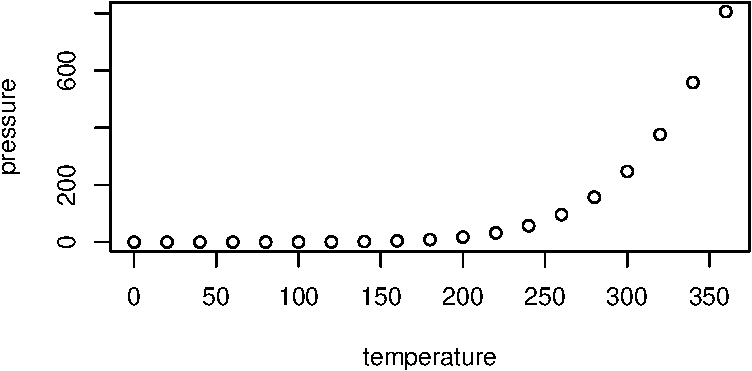
\includegraphics[keepaspectratio]{01-chap1_files/figure-pdf/unnamed-chunk-2-1.pdf}}

Note that the \texttt{\#\textbar{}\ echo:\ false} parameter was added to
the code chunk to prevent printing of the \textbf{R} code that generated
the plot. There are plenty of other ways to add chunk options. More
information is available at
\url{https://quarto.org/docs/computations/execution-options.html}.

Another useful chunk option is the setting of
\texttt{\#\textbar{}\ cache:\ true} as you see here. If document
rendering becomes time consuming due to long computations or plots that
are expensive to generate you can use caching to improve performance.
Later in this file, you'll see a way to reference plots created in
\textbf{R} or external figures.

\section{Loading and exploring data}\label{loading-and-exploring-data}

Included in this template is a file called \texttt{flights.csv}. This
file includes a subset of the larger dataset of information about all
flights that departed from Seattle and Portland in 2014. More
information about this dataset and its \textbf{R} package is available
at \url{http://github.com/ismayc/pnwflights14}. This subset includes
only Portland flights and only rows that were complete with no missing
values. Merges were also done with the \texttt{airports} and
\texttt{airlines} data sets in the \texttt{pnwflights14} package to get
more descriptive airport and airline names.

We can load in this data set using the following command:

\begin{Shaded}
\begin{Highlighting}[]
\NormalTok{flights }\OtherTok{\textless{}{-}} \FunctionTok{read.csv}\NormalTok{(}\StringTok{"data/flights.csv"}\NormalTok{)}
\end{Highlighting}
\end{Shaded}

The data is now stored in the data frame called \texttt{flights} in
\textbf{R}. To get a better feel for the variables included in this
dataset we can use a variety of functions. Here we can see the
dimensions (rows by columns) and also the names of the columns.

\begin{Shaded}
\begin{Highlighting}[]
\FunctionTok{dim}\NormalTok{(flights)}
\end{Highlighting}
\end{Shaded}

\begin{verbatim}
[1] 52808    16
\end{verbatim}

\begin{Shaded}
\begin{Highlighting}[]
\FunctionTok{names}\NormalTok{(flights)}
\end{Highlighting}
\end{Shaded}

\begin{verbatim}
 [1] "month"        "day"          "dep_time"     "dep_delay"    "arr_time"    
 [6] "arr_delay"    "carrier"      "tailnum"      "flight"       "dest"        
[11] "air_time"     "distance"     "hour"         "minute"       "carrier_name"
[16] "dest_name"   
\end{verbatim}

Another good idea is to take a look at the dataset in table form. With
this dataset having more than 50,000 rows, we won't explicitly show the
results of the command here. I recommend you enter the command into the
Console \textbf{\emph{after}} you have run the \textbf{R} chunks above
to load the data into \textbf{R}.

\begin{Shaded}
\begin{Highlighting}[]
\FunctionTok{View}\NormalTok{(flights)}
\end{Highlighting}
\end{Shaded}

While not required, it is highly recommended you use the \texttt{dplyr}
package to manipulate and summarize your data set as needed. It uses a
syntax that is easy to understand using chaining operations. Below I've
created a few examples of using \texttt{dplyr} to get information about
the Portland flights in 2014. You will also see the use of the
\texttt{ggplot2} package, which produces beautiful, high-quality
academic visuals.

We begin by checking to ensure that needed packages are installed and
then we load them into our current working environment:

\begin{Shaded}
\begin{Highlighting}[]
\CommentTok{\# List of packages required for this analysis}
\NormalTok{pkg }\OtherTok{\textless{}{-}} \FunctionTok{c}\NormalTok{(}\StringTok{"dplyr"}\NormalTok{, }\StringTok{"ggplot2"}\NormalTok{, }\StringTok{"knitr"}\NormalTok{)}
\CommentTok{\# Check if packages are not installed and assign the}
\CommentTok{\# names of the packages not installed to the variable new.pkg}
\NormalTok{new.pkg }\OtherTok{\textless{}{-}}\NormalTok{ pkg[}\SpecialCharTok{!}\NormalTok{(pkg }\SpecialCharTok{\%in\%} \FunctionTok{installed.packages}\NormalTok{())]}
\CommentTok{\# If there are any packages in the list that aren\textquotesingle{}t installed,}
\CommentTok{\# install them}
\ControlFlowTok{if}\NormalTok{ (}\FunctionTok{length}\NormalTok{(new.pkg))}
  \FunctionTok{install.packages}\NormalTok{(new.pkg, }\AttributeTok{repos =} \StringTok{"http://cran.rstudio.com"}\NormalTok{)}
\CommentTok{\# Load packages}
\FunctionTok{library}\NormalTok{(dplyr)}
\FunctionTok{library}\NormalTok{(ggplot2)}
\FunctionTok{library}\NormalTok{(knitr)}
\end{Highlighting}
\end{Shaded}

The example we show here does the following:

\begin{itemize}
\item
  Selects only the \texttt{carrier\_name} and \texttt{arr\_delay} from
  the \texttt{flights} dataset and then assigns this subset to a new
  variable called \texttt{flights2}.
\item
  Using \texttt{flights2}, we determine the largest arrival delay for
  each of the carriers.
\end{itemize}

\begin{Shaded}
\begin{Highlighting}[]
\NormalTok{flights2 }\OtherTok{\textless{}{-}}\NormalTok{ flights }\SpecialCharTok{\%\textgreater{}\%}
  \FunctionTok{select}\NormalTok{(carrier\_name, arr\_delay)}
\NormalTok{max\_delays }\OtherTok{\textless{}{-}}\NormalTok{ flights2 }\SpecialCharTok{\%\textgreater{}\%}
  \FunctionTok{group\_by}\NormalTok{(carrier\_name) }\SpecialCharTok{\%\textgreater{}\%}
  \FunctionTok{summarize}\NormalTok{(}\AttributeTok{max\_arr\_delay =} \FunctionTok{max}\NormalTok{(arr\_delay, }\AttributeTok{na.rm =} \ConstantTok{TRUE}\NormalTok{))}
\end{Highlighting}
\end{Shaded}

A useful function in the \texttt{knitr} package for making nice tables
in \emph{Quarto} is called \texttt{kable}. It is much easier to use than
manually entering values into a table by copying and pasting values into
Excel or LaTeX. This again goes to show how nice reproducible documents
can be!

\begin{Shaded}
\begin{Highlighting}[]
\FunctionTok{kable}\NormalTok{(max\_delays,}
      \AttributeTok{col.names =} \FunctionTok{c}\NormalTok{(}\StringTok{"Airline"}\NormalTok{, }\StringTok{"Max Arrival Delay"}\NormalTok{),}
      \AttributeTok{longtable =} \ConstantTok{TRUE}\NormalTok{,}
      \AttributeTok{booktabs =} \ConstantTok{TRUE}\NormalTok{)}
\end{Highlighting}
\end{Shaded}

\begin{longtable}[]{@{}lr@{}}

\caption{\label{tbl-maxdelays}Maximum arrival delays (minutes) by
airline for Portland departures in 2014}

\tabularnewline

\toprule\noalign{}
Airline & Max Arrival Delay \\
\midrule\noalign{}
\endhead
\bottomrule\noalign{}
\endlastfoot
Alaska Airlines Inc. & 338 \\
American Airlines Inc. & 1539 \\
Delta Air Lines Inc. & 651 \\
Frontier Airlines Inc. & 575 \\
Hawaiian Airlines Inc. & 407 \\
JetBlue Airways & 273 \\
SkyWest Airlines Inc. & 421 \\
Southwest Airlines Co. & 694 \\
US Airways Inc. & 347 \\
United Air Lines Inc. & 472 \\
Virgin America & 366 \\

\end{longtable}

The last two options make the table a little easier-to-read.

We can further look into the properties of the largest value here for
American Airlines Inc.~To do so, we can isolate the row corresponding to
the arrival delay of 1539 minutes for American in our original
\texttt{flights} dataset.

\begin{Shaded}
\begin{Highlighting}[]
\NormalTok{flights }\SpecialCharTok{\%\textgreater{}\%}
  \FunctionTok{filter}\NormalTok{(arr\_delay }\SpecialCharTok{==} \DecValTok{1539}\NormalTok{,}
\NormalTok{         carrier\_name }\SpecialCharTok{==} \StringTok{"American Airlines Inc."}\NormalTok{) }\SpecialCharTok{\%\textgreater{}\%}
  \FunctionTok{select}\NormalTok{(}\SpecialCharTok{{-}}\FunctionTok{c}\NormalTok{(month, day, carrier, dest\_name, hour,}
\NormalTok{            minute, carrier\_name, arr\_delay))}
\end{Highlighting}
\end{Shaded}

\begin{verbatim}
  dep_time dep_delay arr_time tailnum flight dest air_time distance
1     1403      1553     1934  N595AA   1568  DFW      182     1616
\end{verbatim}

We see that the flight occurred on March 3rd and departed a little after
2 PM on its way to Dallas/Fort Worth. Lastly, we show how we can
visualize the arrival delay of all departing flights from Portland on
March 3rd against time of departure.

\begin{Shaded}
\begin{Highlighting}[]
\NormalTok{flights }\SpecialCharTok{\%\textgreater{}\%}
  \FunctionTok{filter}\NormalTok{(month }\SpecialCharTok{==} \DecValTok{3}\NormalTok{, day }\SpecialCharTok{==} \DecValTok{3}\NormalTok{) }\SpecialCharTok{\%\textgreater{}\%}
  \FunctionTok{ggplot}\NormalTok{(}\FunctionTok{aes}\NormalTok{(}\AttributeTok{x =}\NormalTok{ dep\_time, }\AttributeTok{y =}\NormalTok{ arr\_delay)) }\SpecialCharTok{+} \FunctionTok{geom\_point}\NormalTok{()}
\end{Highlighting}
\end{Shaded}

\begin{figure}[H]

\centering{

\pandocbounded{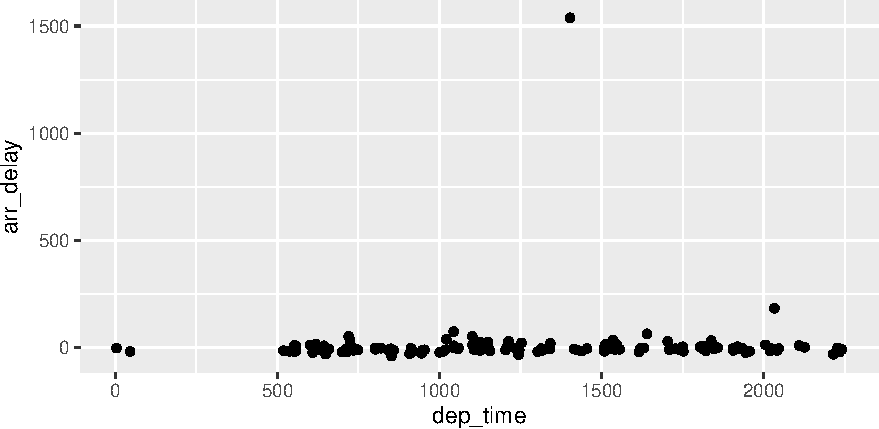
\includegraphics[keepaspectratio]{01-chap1_files/figure-pdf/fig-march3-1.pdf}}

}

\caption[Arrival delay vs.~departure time, March 3,
2014]{\label{fig-march3}Arrival delay (minutes) versus departure time
for all Portland flights on March 3, 2014. Points in the upper right
represent late evening flights that accumulated significant delays
throughout the day.}

\end{figure}%

The \texttt{fig-scap} option provides a short caption that appears in
the List of Figures, while \texttt{fig-cap} provides the full caption
displayed under the figure. Similarly, tables support \texttt{tbl-scap}
for a short List of Tables entry.

\section{Additional resources}\label{additional-resources}

\begin{itemize}
\item
  \emph{Quarto} Documentation - \url{https://quarto.org/docs/guide/}
\item
  \emph{Markdown} Cheatsheet -
  \url{https://github.com/adam-p/markdown-here/wiki/Markdown-Cheatsheet}
\item
  Introduction to \texttt{dplyr} - \url{https://dplyr.tidyverse.org/}
\item
  \texttt{ggplot2} Documentation - \url{https://ggplot2.tidyverse.org/}
\end{itemize}

\bookmarksetup{startatroot}

\chapter{Mathematics and Science}\label{math-sci}

\section{Math}\label{math}

\TeX~is the best way to typeset mathematics. Donald Knuth designed
\TeX~when he got frustrated at how long it was taking the typesetters to
finish his book, which contained a lot of mathematics. One nice feature
of \emph{Quarto} is its ability to read LaTeX code directly.

If you are doing a thesis that will involve lots of math, you will want
to read the following section which has been commented out. If you're
not going to use math, skip over or delete this next commented section.

\section{Chemistry 101: Symbols}\label{chemistry-101-symbols}

Chemical formulas will look best if they are not italicized. Get around
math mode's automatic italicizing in LaTeX by using the argument
\texttt{\$\textbackslash{}mathrm\{formula\ here\}\$}, with your formula
inside the curly brackets. (Notice the use of the backticks here which
enclose text that acts as code.)

So, \(\mathrm{Fe_2^{2+}Cr_2O_4}\) is written
\texttt{\$\textbackslash{}mathrm\{Fe\_2\^{}\{2+\}Cr\_2O\_4\}\$}.

\noindent Exponent or Superscript: \(\mathrm{O^-}\)

\noindent Subscript: \(\mathrm{CH_4}\)

To stack numbers or letters as in \(\mathrm{Fe_2^{2+}}\), the subscript
is defined first, and then the superscript is defined.

\noindent Bullet: CuCl \(\bullet\) \(\mathrm{7H_{2}O}\)

\noindent Delta: \(\Delta\)

\noindent Reaction Arrows: \(\longrightarrow\) or
\(\xrightarrow{solution}\)

\noindent Resonance Arrows: \(\leftrightarrow\)

\noindent Reversible Reaction Arrows: \(\rightleftharpoons\)

\subsection{Typesetting reactions}\label{typesetting-reactions}

You may wish to put your reaction in an equation environment, which
means that LaTeX will place the reaction where it fits and will number
the equations for you.

\begin{equation}\phantomsection\label{eq-reaction}{
\mathrm{C_6H_{12}O_6  + 6O_2} \longrightarrow \mathrm{6CO_2 + 6H_2O}
}\end{equation}

We can reference this combustion of glucose reaction via
Equation~\ref{eq-reaction}.

\subsection{Other examples of
reactions}\label{other-examples-of-reactions}

\(\mathrm{NH_4Cl_{(s)}}\) \(\rightleftharpoons\)
\(\mathrm{NH_{3(g)}+HCl_{(g)}}\)

\noindent \(\mathrm{MeCH_2Br + Mg}\) \(\xrightarrow[below]{above}\)
\(\mathrm{MeCH_2\bullet Mg \bullet Br}\)

\section{Physics}\label{physics}

Many of the symbols you will need can be found on the math page
\url{http://web.reed.edu/cis/help/latex/math.html} and the Comprehensive
LaTeX Symbol Guide
(\url{http://mirror.utexas.edu/ctan/info/symbols/comprehensive/symbols-letter.pdf}).

\section{Biology}\label{biology}

You will probably find the resources at
\url{http://www.lecb.ncifcrf.gov/~toms/latex.html} helpful, particularly
the links to bsts for various journals. You may also be interested in
TeXShade for nucleotide typesetting
(\url{http://homepages.uni-tuebingen.de/beitz/txe.html}). Be sure to
read the proceeding chapter on graphics and tables.

\bookmarksetup{startatroot}

\chapter{Tables, Graphics, References, and Labels}\label{ref-labels}

\section{Tables}\label{tables}

In addition to the tables that can be automatically generated from a
data frame in \textbf{R} that you saw in (\textbf{rmd-basics?}) using
the \texttt{kable} function, you can also create tables using
\emph{pandoc}. (More information is available at
\url{http://pandoc.org/README.html\#tables}.) This might be useful if
you don't have values specifically stored in \textbf{R}, but you'd like
to display them in table form. Below is an example. Pay careful
attention to the alignment in the table and hyphens to create the rows
and columns.

\begin{longtable}[]{@{}
  >{\centering\arraybackslash}p{(\linewidth - 4\tabcolsep) * \real{0.3133}}
  >{\centering\arraybackslash}p{(\linewidth - 4\tabcolsep) * \real{0.5060}}
  >{\centering\arraybackslash}p{(\linewidth - 4\tabcolsep) * \real{0.1807}}@{}}
\caption{Correlation of Inheritance Factors for Parents and
Child}\label{tbl-inher}\tabularnewline
\toprule\noalign{}
\begin{minipage}[b]{\linewidth}\centering
Factors
\end{minipage} & \begin{minipage}[b]{\linewidth}\centering
Correlation between Parents \& Child
\end{minipage} & \begin{minipage}[b]{\linewidth}\centering
Inherited
\end{minipage} \\
\midrule\noalign{}
\endfirsthead
\toprule\noalign{}
\begin{minipage}[b]{\linewidth}\centering
Factors
\end{minipage} & \begin{minipage}[b]{\linewidth}\centering
Correlation between Parents \& Child
\end{minipage} & \begin{minipage}[b]{\linewidth}\centering
Inherited
\end{minipage} \\
\midrule\noalign{}
\endhead
\bottomrule\noalign{}
\endlastfoot
Education & -0.49 & Yes \\
Socio-Economic Status & 0.28 & Slight \\
Income & 0.08 & No \\
Family Size & 0.18 & Slight \\
Occupational Prestige & 0.21 & Slight \\
\end{longtable}

We can also create a link to the table by doing the following:
Table~\ref{tbl-inher}. If you go back to
\hyperref[loading-and-exploring-data]{Loading and exploring data} and
look at the \texttt{kable} table, we can create a reference to this max
delays table too: Table~\ref{tbl-maxdelays}. The addition of the
\texttt{\{\#tbl-label\}} attribute to the end of the table caption
allows us to then make a reference to the table using
\texttt{@tbl-label}. Note that this reference could appear anywhere
throughout the document after the table has appeared.

We will next explore ways to create this label-ref link using figures.

\clearpage

\section{Figures}\label{figures}

If your thesis has a lot of figures, \emph{Quarto} might behave better
for you than that other word processor. One perk is that it will
automatically number the figures accordingly in each chapter. You'll
also be able to create a label for each figure, add a caption, and then
reference the figure in a way similar to what we saw with tables
earlier. If you label your figures, you can move the figures around and
\emph{Quarto} will automatically adjust the numbering for you. No need
for you to remember!

In the \textbf{R} chunk below, we will load in a picture stored as
\texttt{reed.jpg} in our main directory. We then give it the caption of
``Reed logo'' and the label ``fig-reedlogo''. Make note of the different
\textbf{R} chunk options that are given in the Quarto file (not shown in
the rendered document).

\begin{Shaded}
\begin{Highlighting}[]
\FunctionTok{include\_graphics}\NormalTok{(}\AttributeTok{path =} \StringTok{"figure/reed.jpg"}\NormalTok{)}
\end{Highlighting}
\end{Shaded}

\begin{figure}[H]

\centering{


\includegraphics[width=0.83in,height=\textheight,keepaspectratio]{figure/reed.jpg}

}

\caption{\label{fig-reedlogo}Reed logo}

\end{figure}%

Here is a reference to the Reed logo: Figure~\ref{fig-reedlogo}. Note
the use of the \texttt{fig-} prefix here. By labeling the \textbf{R}
chunk that contains the figure with
\texttt{\#\textbar{}\ label:\ fig-reedlogo}, we can then reference that
figure later as done in the first sentence here. We can also specify the
caption for the figure via the chunk option
\texttt{\#\textbar{}\ fig-cap:}.

\clearpage

Below we will investigate how to save the output of an \textbf{R} plot
and label it in a way similar to that done above. Recall the
\texttt{flights} dataset from (\textbf{rmd-basics?}). (Note that we've
shown a different way to reference a section or chapter here.) We will
next explore a bar graph with the mean flight departure delays by
airline from Portland for 2014. Note also the use of the \texttt{scale}
parameter which is discussed on the next page.

\begin{Shaded}
\begin{Highlighting}[]
\NormalTok{flights }\SpecialCharTok{\%\textgreater{}\%} \FunctionTok{group\_by}\NormalTok{(carrier) }\SpecialCharTok{\%\textgreater{}\%}
  \FunctionTok{summarize}\NormalTok{(}\AttributeTok{mean\_dep\_delay =} \FunctionTok{mean}\NormalTok{(dep\_delay)) }\SpecialCharTok{\%\textgreater{}\%}
  \FunctionTok{ggplot}\NormalTok{(}\FunctionTok{aes}\NormalTok{(}\AttributeTok{x =}\NormalTok{ carrier, }\AttributeTok{y =}\NormalTok{ mean\_dep\_delay)) }\SpecialCharTok{+}
  \FunctionTok{geom\_bar}\NormalTok{(}\AttributeTok{position =} \StringTok{"identity"}\NormalTok{, }\AttributeTok{stat =} \StringTok{"identity"}\NormalTok{, }\AttributeTok{fill =} \StringTok{"red"}\NormalTok{)}
\end{Highlighting}
\end{Shaded}

\begin{figure}[H]

\centering{

\pandocbounded{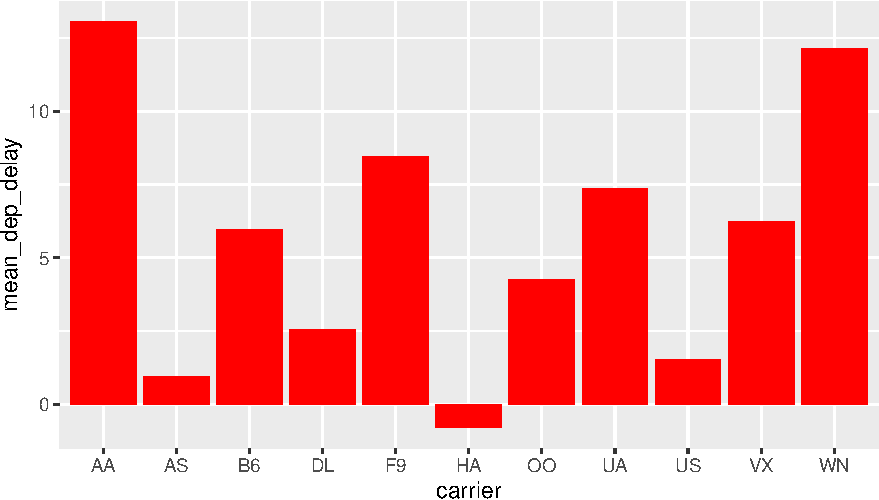
\includegraphics[keepaspectratio]{03-chap3_files/figure-pdf/fig-delaysboxplot-1.pdf}}

}

\caption{\label{fig-delaysboxplot}Mean Delays by Airline}

\end{figure}%

Here is a reference to this image: Figure~\ref{fig-delaysboxplot}.

A table linking these carrier codes to airline names is available at
\url{https://github.com/ismayc/pnwflights14/blob/master/data/airlines.csv}.

\clearpage

Next, we will explore the use of the \texttt{out.extra} chunk option,
which can be used to shrink or expand an image loaded from a file by
specifying \texttt{"scale=\ "}. Here we use the mathematical graph
stored in the ``subdivision.pdf'' file.

\begin{figure}

\centering{

\pandocbounded{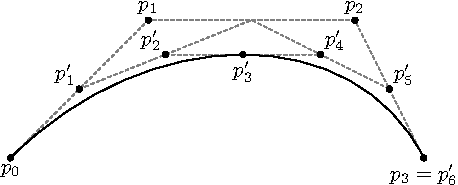
\includegraphics[keepaspectratio]{figure/subdivision.pdf}}

}

\caption{\label{fig-subd}Subdiv. graph}

\end{figure}%

Here is a reference to this image: Figure~\ref{fig-subd}. Note that
\texttt{\#\textbar{}\ echo:\ false} is specified so that the \textbf{R}
code is hidden in the document.

\textbf{More Figure Stuff}

Lastly, we will explore how to rotate and enlarge figures using the
\texttt{out.extra} chunk option. (Currently this only works in the PDF
version of the book.)

\begin{figure}

\centering{

\pandocbounded{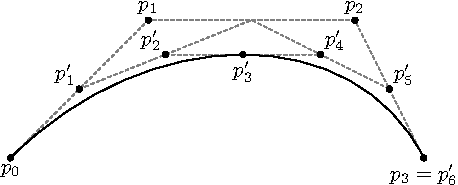
\includegraphics[keepaspectratio]{figure/subdivision.pdf}}

}

\caption{\label{fig-subd2}A Larger Figure, Flipped Upside Down}

\end{figure}%

As another example, here is a reference: Figure~\ref{fig-subd2}.

\section{Footnotes and Endnotes}\label{footnotes-and-endnotes}

You might want to footnote something. \footnote{footnote text} The
footnote will be in a smaller font and placed appropriately. Endnotes
work in much the same way. More information can be found about both on
the CUS site or feel free to reach out to
\href{mailto:data@reed.edu}{\nolinkurl{data@reed.edu}}.

\section{Bibliographies}\label{bibliographies}

Of course you will need to cite things, and you will probably accumulate
an armful of sources. There are a variety of tools available for
creating a bibliography database (stored with the .bib extension). In
addition to BibTeX suggested below, you may want to consider using the
free and easy-to-use tool called Zotero. The Reed librarians have
created Zotero documentation at
\url{http://libguides.reed.edu/citation/zotero}. In addition, a tutorial
is available from Middlebury College at
\url{http://sites.middlebury.edu/zoteromiddlebury/}.

\emph{Quarto} uses \emph{pandoc} (\url{http://pandoc.org/}) to build its
bibliographies. One nice benefit of this is that you won't have to do a
second compile to load in references as standard LaTeX requires. To cite
references in your thesis (after creating your bibliography database),
place the reference name inside square brackets and precede it by the
``at'' symbol. For example, here's a reference to a book about worrying:
(Molina \& Borkovec, 1994). This \texttt{Molina1994} entry appears in a
file called \texttt{thesis.bib} in the \texttt{bib} folder. This
bibliography database file was created by a program called BibTeX. You
can call this file something else if you like (look at the
\texttt{bibliography} setting in \texttt{\_quarto.yml}) and, by default,
it is placed in the \texttt{bib} folder.

For more information about BibTeX and bibliographies, see our CUS site
(\url{http://web.reed.edu/cis/help/latex/index.html})\footnote{Reed~College
  (2007)}. There are three pages on this topic: \emph{bibtex} (which
talks about using BibTeX, at
\url{http://web.reed.edu/cis/help/latex/bibtex.html}),
\emph{bibtexstyles} (about how to find and use the bibliography style
that best suits your needs, at
\url{http://web.reed.edu/cis/help/latex/bibtexstyles.html}) and
\emph{bibman} (which covers how to make and maintain a bibliography by
hand, without BibTeX, at
\url{http://web.reed.edu/cis/help/latex/bibman.html}). The last page
will not be useful unless you have only a few sources.

If you look at the \texttt{\_quarto.yml} file you can see that we can
specify the style of the bibliography by referencing the appropriate csl
file. You can download a variety of different style files at
\url{https://www.zotero.org/styles}. Make sure to download the file into
the csl folder.

\textbf{Tips for Bibliographies}

\begin{itemize}
\tightlist
\item
  Like with thesis formatting, the sooner you start compiling your
  bibliography for something as large as thesis, the better. Typing in
  source after source is mind-numbing enough; do you really want to do
  it for hours on end in late April? Think of it as procrastination.
\item
  The cite key (a citation's label) needs to be unique from the other
  entries.
\item
  When you have more than one author or editor, you need to separate
  each author's name by the word ``and''
  e.g.~\texttt{Author\ =\ \{Noble,\ Sam\ and\ Youngberg,\ Jessica\},}.
\item
  Bibliographies made using BibTeX (whether manually or using a manager)
  accept LaTeX markup, so you can italicize and add symbols as
  necessary.
\item
  To force capitalization in an article title or where all lowercase is
  generally used, bracket the capital letter in curly braces.
\item
  You can add a Reed Thesis citation\footnote{Noble (2002)} option. The
  best way to do this is to use the phdthesis type of citation, and use
  the optional ``type'' field to enter ``Reed thesis'' or
  ``Undergraduate thesis.''
\end{itemize}

\section{Anything else?}\label{anything-else}

If you'd like to see examples of other things in this template, please
contact the Data @ Reed team (email
\href{mailto:data@reed.edu}{\nolinkurl{data@reed.edu}}) with your
suggestions. We love to see people using \emph{Quarto} for their theses,
and are happy to help.

\bookmarksetup{startatroot}

\chapter*{Conclusion}\label{conclusion}
\addcontentsline{toc}{chapter}{Conclusion}

\markboth{Conclusion}{Conclusion}

If we don't want Conclusion to have a chapter number next to it, we can
add the \texttt{\{-\}} attribute.

\textbf{More info}

And here's some other random info: the first paragraph after a chapter
title or section head \emph{shouldn't be} indented, because indents are
to tell the reader that you're starting a new paragraph. Since that's
obvious after a chapter or section title, proper typesetting doesn't add
an indent there.

\appendix

\bookmarksetup{startatroot}

\chapter{The First Appendix}\label{the-first-appendix}

This first appendix includes all of the R chunks of code that were
hidden throughout the document (using the
\texttt{\#\textbar{}\ include:\ false} chunk option) to help with
readability and/or setup.

\textbf{In the Introduction (index.qmd):}

\begin{Shaded}
\begin{Highlighting}[]
\CommentTok{\# Load any R packages you need for your thesis}
\FunctionTok{library}\NormalTok{(knitr)}
\FunctionTok{library}\NormalTok{(ggplot2)}
\end{Highlighting}
\end{Shaded}

\textbf{In (\textbf{ref-labels?}):}

\begin{Shaded}
\begin{Highlighting}[]
\CommentTok{\# Load required packages}
\FunctionTok{library}\NormalTok{(dplyr)}
\FunctionTok{library}\NormalTok{(ggplot2)}
\FunctionTok{library}\NormalTok{(knitr)}
\NormalTok{flights }\OtherTok{\textless{}{-}} \FunctionTok{read.csv}\NormalTok{(}\StringTok{"data/flights.csv"}\NormalTok{)}
\end{Highlighting}
\end{Shaded}

\bookmarksetup{startatroot}

\chapter{The Second Appendix, for
Fun}\label{the-second-appendix-for-fun}

\bookmarksetup{startatroot}

\chapter*{References}\label{references}
\addcontentsline{toc}{chapter}{References}

\markboth{References}{References}

\markboth{References}{References}

% Formatting for bibliography entries
\noindent
\setlength{\parindent}{-0.20in}
\setlength{\leftskip}{0.20in}
\setlength{\parskip}{8pt}

\phantomsection\label{refs}
\begin{CSLReferences}{1}{0}
\bibitem[\citeproctext]{ref-angel2000}
Angel, E. (2000). \emph{Interactive computer graphics : A top-down
approach with OpenGL}. Boston, MA: Addison Wesley Longman.

\bibitem[\citeproctext]{ref-angel2001}
Angel, E. (2001a). \emph{Batch-file computer graphics : A bottom-up
approach with QuickTime}. Boston, MA: Wesley Addison Longman.

\bibitem[\citeproctext]{ref-angel2002a}
Angel, E. (2001b). \emph{Test second book by angel}. Boston, MA: Wesley
Addison Longman.

\bibitem[\citeproctext]{ref-Molina1994}
Molina, S. T., \& Borkovec, T. D. (1994). The {P}enn {S}tate worry
questionnaire: Psychometric properties and associated characteristics.
In G. C. L. Davey \& F. Tallis (Eds.), \emph{Worrying: Perspectives on
theory, assessment and treatment} (pp. 265--283). New York: Wiley.

\bibitem[\citeproctext]{ref-noble2002}
Noble, S. G. (2002). \emph{Turning images into simple line-art}
(Undergraduate thesis). Reed College.

\bibitem[\citeproctext]{ref-reedweb2007}
Reed~College. (2007). LaTeX your document. Retrieved from
\url{http://web.reed.edu/cis/help/LaTeX/index.html}

\end{CSLReferences}




\end{document}
